\chapter{Appendix: Bogolon-mediated electron scattering in 2DEG}\label{AP:CH7}
In this Appendix, we derive the low- and high-temperature $T$-dependencies of the resistivity of a 2D electron gas (2DEG) with parabolic dispersion in a hybrid Bose--Fermi system by extending the Bloch--Gr\"uneisen approach.

%
%------------------
%
\section[Bloch--Gr\"uneisen~formula~for single-bogolon processes]{Bloch-Gr\"uneisen~formula~for single-bogolon\\ processes}
%
Let $f(\mathbf{r},\mathbf{p},t)$ be the electron single-particle distribution function, which depends on coordinate $\mathbf{r}$, particle wave vector $\mathbf{p}$, and time $t$. Its full derivative over time reads
%
\begin{eqnarray}
\frac{df}{dt}=\frac{\partial f}{\partial t}+\frac{\partial f}{\partial \mathbf{r}}\frac{d\mathbf{r}}{dt}
+\frac{\partial f}{\hbar\partial \mathbf{p}}\frac{d\mathbf{p}}{dt}.
\end{eqnarray}
%
Assuming a homogeneous in space distribution of particles ($\partial f/\partial\mathbf{r}=0$), no explicit dependence of the distribution function on time ($\partial f/\partial t=0$), and using Newton's law, we can rewrite the above as
%
\begin{eqnarray}
\frac{df}{dt}=
\mathbf{F}\cdot
\frac{\partial f}{\hbar\partial \mathbf{p}},
\end{eqnarray}
%
where $\mathbf{F}$ is a force acting on the particle.
%
Assuming that the electron is under the influence of the Lorentz force $\mathbf{F}=e_0\mathbf{E}$, where $\mathbf{E}$ is an electric field with kinetics determined by interaction (collisions) with other particles in the media, we find
%
the Boltzmann equation
%
\begin{equation}\label{AP7_Eq1}
e_0\textbf{E}\cdot\frac{\partial f}{\hbar\partial \textbf{p}}=I\{f\},
\end{equation}
%
where the scattering integral in its most generic form is given by~\cite{Zaitsev:2014aa}:
%
\begin{eqnarray}
\label{AP7_Eq2}
I\{f\}&=&-\frac{1}{\hbar}\int\frac{d\textbf{q}d\textbf{p}'}{(2\pi)^2}|M^{(1)}_q|^2\Bigl[N_qf_p(1-f_{p'})\delta(\varepsilon_p-\varepsilon_{p'}+\hbar\omega_q)\delta(\textbf{p}-\textbf{p}'+\textbf{q})\nonumber\\
&{}&{}+(N_q+1)f_p(1-f_{p'})\delta(\varepsilon_p-\varepsilon_{p'}-\hbar\omega_q)\delta(\textbf{p}-\textbf{p}'-\textbf{q})\nonumber \\
&{}&{}+N_qf_{p'}(1-f_{p})\delta(\varepsilon_{p'}-\varepsilon_{p}+\hbar\omega_q)\delta(\textbf{p}'-\textbf{p}+\textbf{q})\nonumber\\
&{}&{}+(N_q+1)f_{p'}(1-f_p)\delta(\varepsilon_{p'}-\varepsilon_{p}-\hbar\omega_q)\delta(\textbf{p}'-\textbf{p}-\textbf{q})\Bigr],
\end{eqnarray}
%
where $M^{(1)}_q=\sqrt{n_c}g_q(u_q+v_q)/L$ is a matrix element of interaction (coming from Eq.~\eqref{CH6_eq.5-a} in the main text), and we consider the fact that the functions $u_q$ and $v_q$ depend on the absolute value of momentum $q$ only.
$N_q$ is a distribution of other particles (to be scattered on), and we use $p\equiv\abs{\mathbf{p}}$.
(Note that the sample length $L$ cancels out in the equation above.)

Further, we take the variations of the integrals in Eq.~\eqref{AP7_Eq2} over $f_p$ and $f_{p'}$ along the method discussed in~\cite{Zaitsev:2014aa}.
For example, let us consider the terms in the square brackets in the first and last lines of Eq.~\eqref{AP7_Eq2}: $N_{\textbf{q}}f_p(1-f_{p'})-(N_{\textbf{q}'}+1)f_{p'}(1-f_{p})$.
Taking a variation over $f_p$, we find:
%
\begin{eqnarray}
\label{EqBol1}
\delta f_p\left\{(1-f_{p^\prime})N_q
+f_{p^\prime}(N_{q}+1)\right\}
=
\delta f_pN_qn_F(\xi_{p'})
    \left(
e^{\frac{\xi_{p'}}{k_BT}}
+e^{\frac{\hbar sq}{k_BT}}
    \right)
,
\end{eqnarray}
%
where we denote the equilibrium Fermi distribution as $n_F(p)\equiv n_F(\xi_p)$ with $\xi_p=\varepsilon_p-\mu$ where $\mu$ is the chemical potential.
In the last equality we also consider energy conservation $\xi_{p}=\xi_{p^{\prime}}-\hbar sq$ (which is legitimate for this particular term).

We then assume that the distribution function of electrons $f_p$ is close to the equilibrium one, thus expanding $f_p=n_F(\xi_p)+\delta f_p=n_F(\xi_p)+(\partial n_F(p)/\partial \xi_p)\phi_p=n_F(\xi_p)+\frac{1}{k_BT}n_F(\xi_p)[1-n_F(\xi_p)]\phi_\mathbf{p}$, where we introduce the correction $\phi_\mathbf{p}$. Then Eq.~\eqref{AP7_Eq2} (after some straightforward algebra with the distribution functions) turns into
%
\begin{eqnarray}
\label{AP7_EqPhi}
\frac{\phi_\mathbf{p}}{k_BT}n_F(p^\prime)(1-n_F(p))
(N_q+1)
=\frac{\phi_\mathbf{p}}{k_BT}
(n_F(p)-n_F(p^\prime))
(N_q+1)N_q.
\end{eqnarray}
%
In a similar fashion, we treat the variation of the first and last lines in Eq.~\eqref{AP7_Eq2} over $f_{p^\prime}$ and find
%
\begin{eqnarray}
\label{AP7_EqPhiPrime1}
-\frac{\phi_{\mathbf{p}^\prime}}{k_BT}
(n_F(p)-n_F(p^\prime))
(N_q+1)N_q.
\end{eqnarray}
%
Taken together, we find the first term (out of two) to enter our target expression:
%
\begin{eqnarray}
-\frac{\phi_\mathbf{p}-\phi_{\mathbf{p}^\prime}}{k_BT}
(n_F(p)-n_F(p'))
(N_q+1)N_q
\delta(\varepsilon_{\textbf{p}'}-\varepsilon_{\textbf{p}}-\hbar\omega_{\textbf{q}}).
\end{eqnarray}
%
Repeating a similar variation procedure with all the other terms in Eq.~\eqref{AP7_Eq2}, we find the total formula:
%
\begin{eqnarray}
\label{AP7_3}
e_0\textbf{E}\cdot\frac{\partial f}{\hbar\partial \textbf{p}}&=&\frac{\hbar e_0}{m}\textbf{E}\cdot\textbf{p}\frac{\partial f^0}{\partial \varepsilon_p}=I\{\phi_\textbf{p}\};\\
%\nonumber
I\{\phi_\textbf{p}\}&=&-\frac{1}{\hbar}\int\frac{d\textbf{q}d\textbf{p}'}{(2\pi)^2}|M^{(1)}_q|^2\frac{1}{\hbar}\frac{\partial N_q}{\partial \omega_q}
\left(f^0(\varepsilon_p)-f^0(\varepsilon_{p'})\right)
\left(\phi_{\textbf{p}}-\phi_{\textbf{p}'}\right) \\ \nonumber
&\times&\Bigl[\delta(\varepsilon_{p}-\varepsilon_{p'}-\hbar\omega_q)\delta(\textbf{p}-\textbf{p}'-\textbf{q})
-\delta(\varepsilon_{p}-\varepsilon_{p'}+\hbar\omega_q)\delta(\textbf{p}-\textbf{p}'+\textbf{q})\Bigr],
\end{eqnarray}
%
where
%
$$\frac{\partial N_q}{\partial \omega_q}=-\frac{\hbar}{k_BT}N_q(1+N_q)$$
%
(which can be checked by direct substitution) and $m$ is the effective electron mass in the 2DEG having the dispersion $\varepsilon_p=\hbar^2p^2/(2m)$.

Further using the wave vector-dependent delta-function, we integrate over the electron wave vector $\textbf{p}'$ and find
%
\begin{eqnarray}
\label{AP7_Eq4}
\frac{\hbar e_0}{m}\textbf{E}\cdot\textbf{p}\frac{\partial f^0}{\partial \varepsilon_p}
=&-&\frac{1}{\hbar}\int\frac{d\textbf{q}}{(2\pi)^2}|M^{(1)}_q|^2\frac{1}{\hbar}\frac{\partial N_q}{\partial \omega_q}
\left(f^0(\varepsilon_p)-f^0(\varepsilon_{p}-\hbar\omega_q)\right)\nonumber \\ \nonumber
&\times& \left(\phi_{\textbf{p}}-\phi_{\textbf{p}-\textbf{q}}\right)
\delta(\varepsilon_{\textbf{p}}-\varepsilon_{\textbf{p}-\textbf{q}}-\hbar\omega_\textbf{q})\\
\nonumber
&+&\frac{1}{\hbar}\int\frac{d\textbf{q}}{(2\pi)^2}|M^{(1)}_q|^2\frac{1}{\hbar}\frac{\partial N_q}{\partial \omega_q}
\left(f^0(\varepsilon_p)-f^0(\varepsilon_{p}+\hbar\omega_q)\right)\\ 
&\times& \left(\phi_{\textbf{p}}-\phi_{\textbf{p}+\textbf{q}}\right)
\delta(\varepsilon_{\textbf{p}}-\varepsilon_{\textbf{p}+\textbf{q}}+\hbar\omega_\textbf{q}).
\end{eqnarray}
%
Without a loss of generality, we set the electric field to be directed along the $x$-axis.
Then the correction function becomes
%
\begin{eqnarray}
\phi_\textbf{p}= \frac{\hbar e_0}{m}E_xp_x\tau(\varepsilon_p),
\end{eqnarray}
%
where $\tau(\varepsilon_p)$ is the relaxation time.
%
Cancelling out $e_0/m$ and several other terms on both the right- and left-hand sides of Eq.~\eqref{AP7_Eq4}, we have
%
\begin{eqnarray}\label{AP7_5}
\hbar p_x\frac{\partial f^0}{\partial \varepsilon_p}
=&-&\frac{1}{\hbar}\int\frac{d\textbf{q}}{(2\pi)^2}|M^{(1)}_q|^2\frac{1}{\hbar}\frac{\partial N_q}{\partial \omega_q}
\left[f^0(\varepsilon_p)-f^0(\varepsilon_{p}-\hbar\omega_q)\right] \\ 
&\times&\left[\frac{p_x}{k_F}\tau(\varepsilon_p)-\frac{p_x-q_x}{k_F}\tau(\varepsilon_p-\hbar\omega_q)\right]
\delta(\varepsilon_{\textbf{p}}-\varepsilon_{\textbf{p}-\textbf{q}}-\hbar\omega_\textbf{q})\nonumber\\
&+&\frac{1}{\hbar}\int\frac{d\textbf{q}}{(2\pi)^2}|M^{(1)}_q|^2\frac{1}{\hbar}\frac{\partial N_q}{\partial \omega_q}
\left[f^0(\varepsilon_p)-f^0(\varepsilon_{p}+\hbar\omega_q)\right] \nonumber\\ 
&\times&\left[\frac{p_x}{k_F}\tau(\varepsilon_p)-\frac{p_x+q_x}{k_F}\tau(\varepsilon_p+\hbar\omega_q)\right]
\delta(\varepsilon_{\textbf{p}}-\varepsilon_{\textbf{p}+\textbf{q}}+\hbar\omega_\textbf{q}).\nonumber
\end{eqnarray}
%
Replacing the relaxation time $\tau(\varepsilon)$ with its energy-averaged value $\tau_0$~\cite{Ziman:2001aa}, thus assuming $\tau(\varepsilon_p)\approx\tau(\varepsilon_p\pm\hbar\omega_q)=\tau_0$, one finds
%
\begin{eqnarray}
\label{AP7_Boltzmann1}
\hbar p_x\frac{\partial f^0}{\partial \varepsilon_p}
=&-&\tau_0\int \frac{d\textbf{q}}{(2\pi)^2}q_x|M^{(1)}_q|^2\frac{1}{\hbar}\frac{\partial N_q}{\partial \omega_q} \\ \nonumber
&\times&\left[f^0(\varepsilon_p)-f^0(\varepsilon_{p}-\hbar\omega_q)\right]
\delta(\varepsilon_{\textbf{p}}-\varepsilon_{\textbf{p}-\textbf{q}}-\hbar\omega_\textbf{q})\\
\nonumber
&-&\tau_0\int \frac{d\textbf{q}}{(2\pi)^2}q_x|M^{(1)}_q|^2\frac{1}{\hbar}\frac{\partial N_q}{\partial \omega_q} \\ \nonumber
&\times&\left[f^0(\varepsilon_p)-f^0(\varepsilon_{p}+\hbar\omega_q)\right]
\delta(\varepsilon_{\textbf{p}}-\varepsilon_{\textbf{p}+\textbf{q}}+\hbar\omega_\textbf{q}).
\end{eqnarray}
%

By denoting the angle between vectors $\textbf{p}$ and $\textbf{q}$ as $\varphi$ and the angle between vectors $\textbf{p}$ and $\textbf{E}$ as $\beta$, we have $q_x=q\cos(\varphi+\beta)$ and $p_x=p\cos\beta$.
Using the substitution technique, the $\varphi$-dependent part of Eq.~\eqref{AP7_Boltzmann1} gives
%
\begin{footnotesize}
\begin{eqnarray}
\label{AP7_Eq19}
    &~&\int_0^{2\pi} d\varphi\cos (\varphi+\beta)\delta(\varepsilon_p-\varepsilon_{|\mathbf{p}\pm\mathbf{q}|}\pm\hbar\omega_q)\\ \nonumber
    &=&\frac{2m}{\hbar^2p}\cos\beta\frac{\left(\mp\frac{q}{2p}+\frac{ms}{\hbar p}\right)\Theta\left[1-\left(\mp\frac{q}{2p}+\frac{ms}{\hbar p}\right)^2\right]}{\sqrt{1-\left(\mp\frac{q}{2p}+\frac{ms}{\hbar p}\right)^2}},
\end{eqnarray}
\end{footnotesize}
%
where $\Theta[x]$ is the Heaviside step function ($\Theta$-function in what follows).
\footnote{The way to derive Eq.~\eqref{AP7_Eq19} is the same as the way we derived Eq.~\eqref{AP6_AEq19}.}

After integrating over the angle $\varphi$, we can integrate Eq.~\eqref{AP7_Boltzmann1} over $\xi_p=\varepsilon_p-\mu$, using
%
\begin{eqnarray}
\int\limits_{-\infty}^{\infty}d\xi_p\frac{\partial f^0}{\partial \varepsilon_p}=-1,\nonumber\\
\int\limits_{-\infty}^{\infty}d\xi_p\left(f^0(\varepsilon_p)-f^0(\varepsilon_{p}\pm\hbar\omega_q)\right)=\pm\hbar\omega_q,
\end{eqnarray}
%
and let all electron wave vectors be on the Fermi surface.
%
%%%%%-----
We find
%
\begin{eqnarray}
\label{AP7_rho1}
\frac{1}{\tau_0}&=&\frac{m\xi_I^2}{\hbar k_F^2M}\frac{1}{k_BT}\int_0^\infty \frac{dq}{(2\pi)^2} \frac{q^3e^{-2ql}}{\epsilon(q)^2}(\Gamma_+-\Gamma_-)_{k_F}N_q(1+N_q),
\end{eqnarray}
%
where the subscript $k_F$ in the expression $(\Gamma_--\Gamma_+)_{k_F}$ means that all the electron wave vectors $p$ are to be substituted by the Fermi value $k_F$.
We also
introduce $\xi_I= e_0^2d\sqrt{n_c}/2\epsilon$ and
%
\begin{eqnarray}
\label{AP7_gamma}
\Gamma_{\pm}=\frac{\left(\mp\frac{q}{2p}+\frac{ms}{\hbar p}\right)\Theta\left[1-\left(\mp\frac{q}{2p}+\frac{ms}{\hbar p}\right)^2\right]}{\sqrt{1-\left(\mp\frac{q}{2p}+\frac{ms}{\hbar p}\right)^2}}.
\end{eqnarray}
%
Here, $\epsilon(q)$ is the static screening given by
%
\begin{eqnarray}
\epsilon(q)=\left(1+\frac{2}{a_Bq}\right)\left(1+\frac{1}{q^2\xi^2}\right),
\end{eqnarray}
%
where $a_B$ is the Bohr radius and, as we recall, $\xi$ is the healing length of the condensate.

We now apply the dimensionless variable introduced in Eq.~\eqref{AP6_Dim},
$u=\frac{\hbar sq}{k_BT}$, into Eq.~\eqref{AP7_rho1} and obtain
%
\begin{eqnarray}
\label{AP7_rho2}
\frac{1}{\tau_0}&=&\frac{m\xi_I^2}{\hbar k_F^2M}\frac{(k_BT)^3}{(\hbar s)^4}\int_0^\infty \frac{du}{(2\pi)^2} \frac{u^3e^{(1-2\tilde{l})u}}{(e^u-1)^2}(\Gamma_+-\Gamma_-)_{k_F},
\end{eqnarray}
%
where $s=10^5$ m/s and $l= 5.0\times 10^{-8}$ m/s, then
%
\begin{eqnarray}
\Tilde{l}=\frac{lk_BT}{\hbar s}\sim\frac{k_BT}{10\mbox{ meV}}.
\end{eqnarray}
%
Note that room temperature is $k_BT_R\sim 26$ meV, so that for far lower temperatures we have $\Tilde{l}\ll 1$.
Hence, we can replace
%
\begin{eqnarray}
\label{AP7_approx1}
e^{(1-2\tilde{l})u}\rightarrow e^u.
\end{eqnarray}
%
%
To keep things general, we instead expand
\begin{eqnarray}
\label{AP7_taylor}
e^{-2\tilde{l}u}=\sum_{n=0}^\infty\frac{(-1)^n(2\tilde{l}u)^n}{n!}.
\end{eqnarray}

Let us now look at the argument of the $\Theta$ function in Eq.~\eqref{AP7_gamma}. Its roots for both the cases are
%
\begin{eqnarray}
q_0=\pm 2k_F-\frac{2ms}{\hbar}\approx\pm2k_F,
\end{eqnarray}
%
which means that the Heaviside theta function is non-zero in the integration range
%
\begin{eqnarray}
0\leq q\lesssim 2k_F,
\end{eqnarray}
%
or in terms of $u$,
%
\begin{eqnarray}
\label{AP7_lambda}
0\leq u<\frac{T_\textrm{BG}}{T}\equiv\Lambda,
\end{eqnarray}
%
where $T_\textrm{BG}=2\hbar sk_F/k_B$ is the Bloch--Gr\"{u}neisen temperature for bogolons.

For large $u$ (or $q$), the factors $\Gamma_\pm$ in Eq.~\eqref{AP7_rho2} approach constant values.
In the meantime, the term $u^4\exp({-u})$ rapidly goes to zero for $u>10$.
%
Therefore, we can remove the $\Theta$ function in Eq.~\eqref{AP7_gamma} and only incur a small (imaginary) error.

The term inside the square root of Eq.~\eqref{AP7_gamma} can be rewritten as
%
\begin{eqnarray}
\label{AP7_sqrt}
1-\left(\mp\frac{q}{2p}+\frac{ms}{\hbar p}\right)^2&\approx &\frac{1}{4k_F^2}(2k_F-q)(2k_F+q)\nonumber\\
&=&\left(\frac{k_BT}{2k_F\hbar s}\right)^2(\Lambda-u)(\Lambda+u),
\end{eqnarray}
%
where $\Lambda$ depends on $T$, as was defined in Eq.~\eqref{AP7_lambda}. However, for $T\ll T_\textrm{BG}$, due to the factor $\exp({-u})$, we can simply replace $\Lambda\sim 10$ (or greater) without significantly affecting the result.

The resistivity is inversely proportional to the scattering time. Using Eqs.~\eqref{AP7_taylor} and~\eqref{AP7_sqrt}, and the arguments presented above allowing us to remove the $\Theta$ function, we find
%
\begin{eqnarray}
\label{AP7_28}
\rho^{(1)}=\frac{\pi\hbar^3\xi_I^2}{e_0^2ME_F}\sum_{n=0}^\infty\frac{(-2)^nl^n\gamma_n}{n!(\hbar s)^{n+4}}(k_BT)^{n+4},
% \rho=\frac{\pi\hbar^2}{e_0^2E_F}\frac{1}{\tau_0}=\frac{\pi\hbar^3\xi_I^2\xi^6}{4e_0^2ME_F}\sum_{n=0}^\infty\frac{(-2)^nl^n\gamma_n}{n!(\hbar s)^{n+10}}(k_BT)^{n+9},
\end{eqnarray}
%
where
%
\begin{eqnarray}
\label{AP7_EqMath}
\gamma_n=\int_0^\Lambda\frac{du}{(2\pi)^2}\frac{e^uu^{n+3}}{(e^u-1)^2\sqrt{(\Lambda-u)(\Lambda+u)}}.
\end{eqnarray}
%

This dimensionless integral can be evaluated in closed form when we note that (i) $\Lambda\gg 1$, and (ii) due to the exponential factors in the integrand, the relevant contribution to the integral comes from $0<u\lesssim 1$, so that
%
\begin{eqnarray}
\label{AP7_EqMath2}
\gamma_n\approx\frac{1}{\Lambda}\int_0^\infty\frac{du}{(2\pi)^2}\frac{e^uu^{n+3}}{(e^u-1)^2}=\frac{(n+3)!}{(2\pi)^2}\zeta(n+9)\frac{T}{T_\textrm{BG}}.
\end{eqnarray}
%
The leading term in Eq.~\eqref{AP7_28} if $T\ll T_\textrm{BG}$ reads
%
\begin{eqnarray}
\label{AP7_rho1b}
\rho^{(1)}\approx\frac{\pi\hbar^3\xi_I^2}{e_0^2ME_F}\frac{3!\zeta(3)}{(2\pi)^2k_BT_\textrm{BG}}\left(\frac{k_BT}{\hbar s}\right)^4,
\end{eqnarray}
%
and hence the single-bogolon resistivity behaves as $\rho^{(1)}\propto T^4$ at low temperatures.

%----------------------------
%----------------------------
%----------------------------

\section{Bloch--Gr\"uneisen formula for two-bogolon processes}
The starting equation here is similar to Eq.~\eqref{AP7_Eq1}:
%
\begin{eqnarray}
\nonumber
e_0\mathbf{E}\cdot\frac{df_p}{\hbar d\mathbf{p}}=I\{f_p\}.
\end{eqnarray}
%
We consider the Hamiltonian
Eq.~\eqref{CH6_eq.5-b} from the main text:
%
\begin{equation}\label{1}
V_2=\frac{1}{L^2}\sum_{\mathbf{k},\mathbf{p}',\mathbf{q},\mathbf{q}'}
g_\textbf{k}
c^+_{\textbf{p}'}c_{\textbf{p}}\varphi^+_{\textbf{q}'}\varphi_{\textbf{q}},
%\delta(\textbf{p}'-\textbf{p}-\textbf{k})\delta(\textbf{q}'-\textbf{q}+\textbf{k}),
\end{equation}
%
where
%
\begin{eqnarray}\label{AP7_2}
\varphi^+_{\textbf{q}'}\varphi_{\textbf{q}}&=&(u_{\textbf{q}'}b^+_{\textbf{q}'}+v_{\textbf{q}'}b_{-\textbf{q}'})
(u_{\textbf{q}}b_{\textbf{q}}+v_{\textbf{q}}b^+_{-\textbf{q}})\\ \nonumber
%=\\\nonumber
&=&u_{\textbf{q}'}b^+_{\textbf{q}'}u_{\textbf{q}}b_{\textbf{q}}+u_{\textbf{q}'}b^+_{\textbf{q}'}v_{\textbf{q}}b^+_{-\textbf{q}}+
v_{\textbf{q}'}b_{-\textbf{q}'}u_{\textbf{q}}b_{\textbf{q}}+v_{\textbf{q}'}b_{-\textbf{q}'}v_{\textbf{q}}b^+_{-\textbf{q}}.
\end{eqnarray}
%
Thus, the collision integral reads $I\{f_p\}=I_1-I_2$, where
%
\begin{footnotesize}
\begin{eqnarray}\label{AP7_I1I2}
I_1&=&-\sum_{\mathbf{k},\mathbf{p}',\mathbf{q},\mathbf{q}'}|g_\textbf{k}|^2f_p(1-f_{p'})\delta(\textbf{p}'-\textbf{p}-\textbf{k})\delta(\textbf{q}'-\textbf{q}+\textbf{k})\times\\\nonumber
&\times&\Bigl[u^2_{\textbf{q}'}u^2_{\textbf{q}}(N_{\textbf{q}'}+1)N_{\textbf{q}}
\delta(\varepsilon_{\textbf{p}'}-\varepsilon_{\textbf{p}}+\omega_{\textbf{q}'}-\omega_{\textbf{q}})
+u^2_{\textbf{q}'}v^2_{\textbf{q}}(N_{\textbf{q}'}+1)(N_{-\textbf{q}}+1)
\delta(\varepsilon_{\textbf{p}'}-\varepsilon_{\textbf{p}}+\omega_{\textbf{q}'}+\omega_{-\textbf{q}})\\\nonumber
&+&v^2_{\textbf{q}'}u^2_{\textbf{q}}N_{-\textbf{q}'}N_{\textbf{q}}
\delta(\varepsilon_{\textbf{p}'}-\varepsilon_{\textbf{p}}-\omega_{-\textbf{q}'}-\omega_{\textbf{q}})
+v^2_{\textbf{q}'}v^2_{\textbf{q}}N_{-\textbf{q}'}(N_{-\textbf{q}}+1)
\delta(\varepsilon_{\textbf{p}'}-\varepsilon_{\textbf{p}}-\omega_{-\textbf{q}'}+\omega_{-\textbf{q}})\Bigr],\\
\nonumber
I_2&=&-\sum_{\mathbf{k},\mathbf{p}',\mathbf{q},\mathbf{q}'}|g_\textbf{k}|^2f_{p'}(1-f_{p})\delta(\textbf{p}-\textbf{p}'-\textbf{k})\delta(\textbf{q}'-\textbf{q}+\textbf{k})\times\\\nonumber
&\times&\Bigl[u^2_{\textbf{q}'}u^2_{\textbf{q}}(N_{\textbf{q}'}+1)N_{\textbf{q}}
\delta(\varepsilon_{\textbf{p}}-\varepsilon_{\textbf{p}'}+\omega_{\textbf{q}'}-\omega_{\textbf{q}})
+u^2_{\textbf{q}'}v^2_{\textbf{q}}(N_{\textbf{q}'}+1)(N_{-\textbf{q}}+1)
\delta(\varepsilon_{\textbf{p}}-\varepsilon_{\textbf{p}'}+\omega_{\textbf{q}'}+\omega_{-\textbf{q}})\\\nonumber
&+&v^2_{\textbf{q}'}u^2_{\textbf{q}}N_{-\textbf{q}'}N_{\textbf{q}}
\delta(\varepsilon_{\textbf{p}}-\varepsilon_{\textbf{p}'}-\omega_{-\textbf{q}'}-\omega_{\textbf{q}})
+v^2_{\textbf{q}'}v^2_{\textbf{q}}N_{-\textbf{q}'}(N_{-\textbf{q}}+1)
\delta(\varepsilon_{\textbf{p}}-\varepsilon_{\textbf{p}'}-\omega_{-\textbf{q}'}+\omega_{-\textbf{q}})\Bigr],
\end{eqnarray}
\end{footnotesize}
%
where we assume that $N_\mathbf{x}$ are equilibrium Bose distribution functions. In $I_2$ we can change the signs of the vectors: $\textbf{k}\rightarrow-\textbf{k},\,\textbf{q}\rightarrow-\textbf{q},\,\textbf{q}'\rightarrow-\textbf{q}'$. Taking into account that the distribution functions and energies only depend on the absolute value of the wave vectors, we find
%
\begin{footnotesize}
\begin{eqnarray}
I_1&=&-\sum_{\mathbf{k},\mathbf{p}',\mathbf{q},\mathbf{q}'}|g_\textbf{k}|^2f_p(1-f_{p'})\delta(\textbf{p}'-\textbf{p}-\textbf{k})\delta(\textbf{q}'-\textbf{q}+\textbf{k})\times\\\nonumber
&\times&\Bigl[u^2_{\textbf{q}'}u^2_{\textbf{q}}(N_{\textbf{q}'}+1)N_{\textbf{q}}
\delta(\varepsilon_{\textbf{p}'}-\varepsilon_{\textbf{p}}+\omega_{\textbf{q}'}-\omega_{\textbf{q}})
+u^2_{\textbf{q}'}v^2_{\textbf{q}}(N_{\textbf{q}'}+1)(N_{\textbf{q}}+1)
\delta(\varepsilon_{\textbf{p}'}-\varepsilon_{\textbf{p}}+\omega_{\textbf{q}'}+\omega_{\textbf{q}})\\\nonumber
&+&v^2_{\textbf{q}'}u^2_{\textbf{q}}N_{\textbf{q}'}N_{\textbf{q}}
\delta(\varepsilon_{\textbf{p}'}-\varepsilon_{\textbf{p}}-\omega_{\textbf{q}'}-\omega_{\textbf{q}})
+v^2_{\textbf{q}'}v^2_{\textbf{q}}N_{\textbf{q}'}(N_{\textbf{q}}+1)
\delta(\varepsilon_{\textbf{p}'}-\varepsilon_{\textbf{p}}-\omega_{\textbf{q}'}+\omega_{\textbf{q}})\Bigr],\\
\nonumber
I_2&=&-\sum_{\mathbf{k},\mathbf{p}',\mathbf{q},\mathbf{q}'}|g_\textbf{k}|^2f_{p'}(1-f_{p})\delta(-\textbf{p}+\textbf{p}'+\textbf{k})\delta(-\textbf{q}'+\textbf{q}-\textbf{k})\times\\\nonumber
&\times&\Bigl[u^2_{\textbf{q}'}u^2_{\textbf{q}}(N_{\textbf{q}'}+1)N_{\textbf{q}}
\delta(\varepsilon_{\textbf{p}}-\varepsilon_{\textbf{p}'}+\omega_{\textbf{q}'}-\omega_{\textbf{q}})
+u^2_{\textbf{q}'}v^2_{\textbf{q}}(N_{\textbf{q}'}+1)(N_{\textbf{q}}+1)
\delta(\varepsilon_{\textbf{p}}-\varepsilon_{\textbf{p}'}+\omega_{\textbf{q}'}+\omega_{\textbf{q}})\\\nonumber
&+&v^2_{\textbf{q}'}u^2_{\textbf{q}}N_{\textbf{q}'}N_{\textbf{q}}
\delta(\varepsilon_{\textbf{p}}-\varepsilon_{\textbf{p}'}-\omega_{\textbf{q}'}-\omega_{\textbf{q}})
+v^2_{\textbf{q}'}v^2_{\textbf{q}}N_{\textbf{q}'}(N_{\textbf{q}}+1)
\delta(\varepsilon_{\textbf{p}}-\varepsilon_{\textbf{p}'}-\omega_{\textbf{q}'}+\omega_{\textbf{q}})\Bigr].
\end{eqnarray}
\end{footnotesize}
%
We see that the delta-functions describing the momentum conservation are the same. We also use that for the linear spectrum of bogolons,  $u^2_{\textbf{q}'}u^2_{\textbf{q}}=u^2_{\textbf{q}'}v^2_{\textbf{q}}=v^2_{\textbf{q}'}v^2_{\textbf{q}}=v^2_{\textbf{q}'}v^2_{\textbf{q}}$.
This yields:
%
\begin{footnotesize}
\begin{eqnarray}\label{APL_5}
I_1-I_2&=&-\sum_{\mathbf{k},\mathbf{p}',\mathbf{q},\mathbf{q}'}u^2_{\textbf{q}'}u^2_{\textbf{q}}|g_\textbf{k}|^2\delta(\textbf{p}'-\textbf{p}-\textbf{k})\delta(\textbf{q}'-\textbf{q}+\textbf{k})\\ \nonumber
&\times&  \Bigr[N_{\textbf{q}'}N_{\textbf{q}}f_p(1-f_{p'})-(N_{\textbf{q}'}+1)(N_{\textbf{q}}+1)f_{p'}(1-f_{p})\Bigl] \delta(\varepsilon_{\textbf{p}'}-\varepsilon_{\textbf{p}}-\omega_{\textbf{q}'}-\omega_{\textbf{q}})\\ \nonumber
&+&\Bigl[(N_{\textbf{q}'}+1)(N_{\textbf{q}}+1)f_p(1-f_{p'})-N_{\textbf{q}'}N_{\textbf{q}}f_{p'}(1-f_{p})\Bigr] \delta(\varepsilon_{\textbf{p}'}-\varepsilon_{\textbf{p}}+\omega_{\textbf{q}'}+\omega_{\textbf{q}})\\\nonumber
&+&\Bigr[N_{\textbf{q}'}(N_{\textbf{q}}+1)f_p(1-f_{p'})-(N_{\textbf{q}'}+1)N_{\textbf{q}}f_{p'}(1-f_{p})\Bigl] \delta(\varepsilon_{\textbf{p}'}-\varepsilon_{\textbf{p}}-\omega_{\textbf{q}'}+\omega_{\textbf{q}})\\\nonumber
&+&\Bigl[(N_{\textbf{q}'}+1)N_{\textbf{q}}f_p(1-f_{p'})-N_{\textbf{q}'}(N_{\textbf{q}}+1)f_{p'}(1-f_{p})\Bigr] \delta(\varepsilon_{\textbf{p}'}-\varepsilon_{\textbf{p}}+\omega_{\textbf{q}'}-\omega_{\textbf{q}}) .
\end{eqnarray}
\end{footnotesize}
%

The sums in Eq.~\eqref{APL_5} can be replaced by integrals in the continuous limit, as discussed in Eq.~\eqref{AP7_Eq2} for the single-bogolon case and~\cite{Zaitsev:2014aa}.
% Then we can consider variations of such integrals over $f_p$ and $f_{p^\prime}$~\cite{Zaitsev:2014aa}.
For example, let us consider the terms in the square brackets in the second line of Eq.~\eqref{APL_5}: $N_{\textbf{q}'}N_{\textbf{q}}f_p(1-f_{p'})-(N_{\textbf{q}'}+1)(N_{\textbf{q}}+1)f_{p'}(1-f_{p})$.
Taking a variation over $f_p$ we have:
%
\begin{eqnarray}
\label{EqBol}
&{}&{}\delta f_p\left\{(1-f_{p^\prime})N_qN_{q^\prime}+f_{p^\prime}(N_q+1)(N_{q^\prime}+1)\right\}\\ \nonumber
&=& \delta f_pN_qN_{q^\prime}n_F(p^\prime)\left\{\exp\left(\frac{\xi_{p^{\prime}}}{k_BT}\right)+\exp\left(\frac{\hbar s (q+q^\prime)}{k_BT}\right)\right\}\\ \nonumber
&=&\delta f_pN_qN_{q^\prime}n_F(p^\prime) \exp\left(\frac{\hbar s (q+q^\prime)}{k_BT}\right) \left\{\exp\left(\frac{\xi_{p^{\prime}}-\hbar s (q+q^\prime)}{k_BT}\right)+1\right\}\\ \nonumber
&=& \delta f_p(N_q+1)(N_{q^\prime}+1)n_F(p^\prime)\frac{1}{n_F(p)},
\end{eqnarray}
%
where w$n_F(p)\equiv n_F(\xi_p)$ is the equilibrium Fermi distribution. In the last equality, we also use the energy conservation $\xi_{p}=\xi_{p^{\prime}}-\hbar s (q+q^\prime)$.

We assume that the distribution function of electrons $f_p$ is close to the equilibrium distribution, thus expanding $f_p=n_F(\xi_p)+\delta f_p=n_F(\xi_p)+(\partial n_F(p)/\partial \xi_p)\phi_p=n_F(\xi_p)+\frac{1}{k_BT}n_F(\xi_p)[1-n_F(\xi_p)]\phi_p$, where we introduce the correction $\phi_p$. Then Eq.~\eqref{EqBol} turns into
%
\begin{eqnarray}
\label{AP7_EqPhi2}
&{}&{}\frac{\phi_p}{k_BT}n_F(p)(1-n_F(p))
(N_q+1)(N_{q^\prime}+1)n_F(p^\prime)\frac{1}{n_F(p)}\\\nonumber
&=&\frac{\phi_p}{k_BT}(n_F(p)-n_F(p^\prime))
(N_q+1)(N_{q^\prime}+1)N_{q+q^\prime}.
\end{eqnarray}
%

We similarly treat the variation of the first line in Eq.~\eqref{APL_5}  over $f_{p^\prime}$ and find
%
\begin{eqnarray}
\label{AP7_EqPhiPrime2}
-\frac{\phi_{p^\prime}}{k_BT}(n_F(p)-n_F(p^\prime))
N_qN_{q^\prime}(N_{q+q^\prime}+1).
\end{eqnarray}
%
Discovering that $N_qN_{q^\prime}(N_{q+q^\prime}+1)=(N_q+1)(N_{q^\prime}+1)N_{q+q^\prime}$, which means that $\phi_p$ and $\phi_{p^\prime}$ in Eqs.~\eqref{AP7_EqPhi2} and~\eqref{AP7_EqPhiPrime2} have equivalent prefactors, we find the first term (out of four) to enter our target expression:
%
\begin{eqnarray}
-\frac{\phi_p-\phi_{p^\prime}}{k_BT}(n_F(p)-n_F(p^\prime))
N_qN_{q^\prime}(N_{q+q^\prime}+1)\delta(\varepsilon_{\textbf{p}'}-\varepsilon_{\textbf{p}}-\omega_{\textbf{q}'}-\omega_{\textbf{q}}).
\end{eqnarray}
%

Repeating a similar variation procedure with all the other terms in Eq.~\eqref{APL_5}, we find the total formula:
%
\begin{gather}\label{EqZaiatz}
I_1-I_2=-\sum_{\mathbf{k},\mathbf{p}',\mathbf{q},\mathbf{q}'}u^2_{\textbf{q}'}u^2_{\textbf{q}}|g_\textbf{k}|^2
\frac{\phi_{\mathbf{p}}-\phi_{\mathbf{p^\prime}}}{k_BT}
[n_F(\mathbf{p})-n_F(\mathbf{p}^\prime)]
\delta(\textbf{p}'-\textbf{p}-\textbf{k})\delta(\textbf{q}'-\textbf{q}+\textbf{k})\\
\nonumber
\times
\{
N_{q}N_{q^\prime}(N_{q+q^\prime}+1)
\Bigr[\delta(\varepsilon_{\textbf{p}'}-\varepsilon_{\textbf{p}}-\omega_{\textbf{q}'}-\omega_{\textbf{q}})
-
\delta(\varepsilon_{\textbf{p}'}-\varepsilon_{\textbf{p}}+\omega_{\textbf{q}'}+\omega_{\textbf{q}})\Bigl]+\\
\nonumber
+
(N_{q}+1)N_{q^\prime}(N_{q^\prime-q}+1)
\Bigr[\delta(\varepsilon_{\textbf{p}'}-\varepsilon_{\textbf{p}}-\omega_{\textbf{q}'}+\omega_{\textbf{q}})
-
\delta(\varepsilon_{\textbf{p}'}-\varepsilon_{\textbf{p}}+\omega_{\textbf{q}'}-\omega_{\textbf{q}})\Bigl]
\}.
\end{gather}
%

This expression can be presented in the form
%
\begin{gather}\label{6}
I_1-I_2=-\sum_{\mathbf{k},\mathbf{p}'}|g_\textbf{k}|^2\frac{\phi_{\mathbf{p}}-\phi_{\mathbf{p^\prime}}}{k_BT}
[n_F(\mathbf{p})-n_F(\mathbf{p}^\prime)]
\delta(\textbf{p}'-\textbf{p}-\textbf{k})\int d \epsilon \delta(\varepsilon_{\textbf{p}'}-\varepsilon_{\textbf{p}}-\epsilon)F(\textbf{k},\epsilon),\\\nonumber
F(\textbf{k},\epsilon)=\sum_{\mathbf{q},\mathbf{q}'} u^2_{\textbf{q}'}u^2_{\textbf{q}}
\delta(\textbf{q}'-\textbf{q}+\textbf{k})
\Bigl(
N_{q}N_{q^\prime}(N_{q+q^\prime}+1)
\Bigl[\delta(\epsilon-\omega_{\textbf{q}'}-\omega_{\textbf{q}})
-
\delta(\epsilon+\omega_{\textbf{q}'}+\omega_{\textbf{q}})\Bigl]+\\
\nonumber
+
(N_{q}+1)N_{q^\prime}(N_{q^\prime-q}+1)
\Bigr[\delta(\epsilon-\omega_{\textbf{q}'}+\omega_{\textbf{q}})
-
\delta(\epsilon+\omega_{\textbf{q}'}-\omega_{\textbf{q}})\Bigr]
\Bigr).
\end{gather}
%
Now we can integrate over $\textbf{p}',\textbf{q}'$. Using the momentum-conserving delta functions, we find:
%
\begin{gather}\label{7}
I=-\sum_{\mathbf{k}}\int d \epsilon |g_\textbf{k}|^2\frac{\phi_{\mathbf{p}}-\phi_{\textbf{p}+\textbf{k}}}{T}
[n_F(\varepsilon_{\textbf{p}})-n_F(\varepsilon_{\textbf{p}}+\epsilon)]
 \delta(\varepsilon_{\textbf{p}+\textbf{k}}-\varepsilon_{\textbf{p}}-\epsilon)F(\textbf{k},\epsilon);\\\nonumber
F(\textbf{k},\epsilon)=\sum_{\mathbf{q}} u^2_{|\textbf{q}-\textbf{k}|}u^2_{\textbf{q}}
\Bigl(
N_{q}N_{|\textbf{q}-\textbf{k}|}(N_{q+|\textbf{q}-\textbf{k}|}+1)
\Bigl[\delta(\epsilon-\omega_{|\textbf{q}-\textbf{k}|}-\omega_{\textbf{q}})
-
\delta(\epsilon+\omega_{|\textbf{q}-\textbf{k}|}+\omega_{\textbf{q}})\Bigl]+\\
\nonumber
+
(N_{q}+1)N_{|\textbf{q}-\textbf{k}|}(N_{|\textbf{q}-\textbf{k}|-q}+1)
\Bigr[\delta(\epsilon-\omega_{|\textbf{q}-\textbf{k}|}+\omega_{\textbf{q}})
-
\delta(\epsilon+\omega_{|\textbf{q}-\textbf{k}|}-\omega_{\textbf{q}})\Bigr]
\Bigr).
\end{gather}
%
Let us consider the function $F(\mathbf{k},\epsilon)$. We make a replacement $\mathbf{q}\rightarrow \mathbf{q}+\mathbf{k}$ to find:
%
\begin{gather}
F(\textbf{k},\epsilon)=\sum_{\mathbf{q}} u^2_{q}u^2_{|\textbf{q}+\textbf{k}|}
\Bigl\{
N_{|\textbf{q}+\textbf{k}|}N_{q}(N_{|\textbf{q}+\textbf{k}|+q}+1)
\Bigl[\delta(\epsilon-\omega_{q}-\omega_{|\textbf{q}+\textbf{k}|})
-
\delta(\epsilon+\omega_{q}+\omega_{|\textbf{q}+\textbf{k}|})\Bigl]+\\
\nonumber
+
(N_{|\textbf{q}+\textbf{k}|}+1)N_{q}(N_{q-|\textbf{q}+\textbf{k}|}+1)
\Bigr[\delta(\epsilon-\omega_{q}+\omega_{|\textbf{q}+\textbf{k}|})
-
\delta(\epsilon+\omega_{q}-\omega_{|\textbf{q}+\textbf{k}|})\Bigr]
\Bigr\}.
\end{gather}
%
Furthermore, we switch from summation to integration $\sum_{\mathbf{q}}\rightarrow\int d\mathbf{q}$, and we introduce a new variable $q_1=|\textbf{q}+\textbf{k}|$.
Then in $\int d\mathbf{q}$ we will integrate over $q$ and $q_1$ instead of $q$ and the angle between the vectors, using
%
\begin{eqnarray}
\int\frac{d\mathbf{q}}{2\pi}=\frac{4}{(2\pi)^2}\int_0^\infty qdq\int_{|q-k|}^{q+k}q_1dq_1
\frac{1}{\sqrt{[(q+k)^2-q_1^2][q_1^2-(q-k)^2]}}.
\end{eqnarray}
%

This gives
%
\begin{gather}
F(\textbf{k},\epsilon)=\frac{4}{(2\pi)^2}\int_0^\infty
qdq 
u^2_{q}
\int_{|q-k|}^{q+k}
q_1dq_1
u^2_{q_1}
\frac{1}{\sqrt{[(q+k)^2-q_1^2][q_1^2-(q-k)^2]}}\\
\nonumber
\times\Bigl\{
N_{q_1}N_{q}(N_{q_1+q}+1)
\Bigl[\delta(\epsilon-\omega_{q}-\omega_{q_1})
-
\delta(\epsilon+\omega_{q}+\omega_{q_1})\Bigl]+\\
\nonumber
+
(N_{q_1}+1)N_{q}(N_{q-q_1}+1)
\Bigr[\delta(\epsilon-\omega_{q}+\omega_{q_1})
-
\delta(\epsilon+\omega_{q}-\omega_{q_1})\Bigr]
\Bigr\}.
\end{gather}
%
Now we can use the definitions of $u_q$~\cite{Giorgini:1998aa} and linear bogolon dispersion to find:
%
\begin{gather}
F(\textbf{k},\epsilon)=\frac{4}{(2\pi)^2}\frac{(ms)^2}{4}
\int_0^\infty dq 
\int_{|q-k|}^{q+k} dq_1
\frac{1}{\sqrt{[(q+k)^2-q_1^2][q_1^2-(q-k)^2]}}\\
\nonumber
\times
\Bigl\{
N_{q_1}N_{q}(N_{q_1+q}+1)
\Bigl[\delta(\epsilon-s(q+q_1))
-
\delta(\epsilon+s(q+q_1))\Bigl]+\\
\nonumber
+
(N_{q_1}+1)N_{q}(N_{q-q_1}+1)
\Bigr[\delta(\epsilon-s(q-q_1))
-
\delta(\epsilon+s(q-q_1))\Bigr]
\Bigr\}.
\end{gather}
%
For convenience we denote new variables $x=s(q+q_1)$ and $y=-s(q-q_1)$, and we introduce the cut-off $sL^{-1}$ in the integrals. This infrared cut-off is necessary for the convergence of the final integral, as will become clear later on. We emphasize that this cut-off has a physical grounding: it means that the momentum integration cannot include fluctuations with wavelengths larger than the sample size $L$. This yields
%
\begin{gather}
F(\textbf{k},\epsilon)=\frac{1}{2}\left(\frac{ms}{2\pi}\right)^2
\int_{sk+sL^{-1}}^\infty \frac{dx}{\sqrt{x^2-s^2k^2}}
\int_{-sk+sL^{-1}}^{sk-sL^{-1}} \frac{dy}{\sqrt{s^2k^2-y^2}}
\\
\nonumber
\times
\Bigl\{
N\left(\frac{x+y}{2s}\right)N\left(\frac{x-y}{2s}\right)(N\left(\frac{x}{s}\right)+1)
\Bigl[\delta(\epsilon-x)
-
\delta(\epsilon+x)\Bigl]+\\
\nonumber
+
(N\left(\frac{x+y}{2s}\right)+1)N\left(\frac{x-y}{2s}\right)(N\left(\frac{-y}{s}\right)+1)
\Bigr[\delta(\epsilon+y)
-
\delta(\epsilon-y)\Bigr]
\Bigr\}.
\end{gather}
%
We exchange $y\rightarrow-y$ to find:
%
\begin{gather}
F(\textbf{k},\epsilon)=\frac{1}{2}\left(\frac{ms}{2\pi}\right)^2
\int_{sk+sL^{-1}}^\infty \frac{dx}{\sqrt{x^2-s^2k^2}}
\int_{-sk+sL^{-1}}^{sk-sL^{-1}} \frac{dy}{\sqrt{s^2k^2-y^2}}
\\
\nonumber
\times
\Bigl\{
N\left(\frac{x+y}{2s}\right)N\left(\frac{x-y}{2s}\right)(N\left(\frac{x}{s}\right)+1)
\Bigl[\delta(\epsilon-x)
-
\delta(\epsilon+x)\Bigl]+\\
\nonumber
+
(N\left(\frac{x-y}{2s}\right)+1)N\left(\frac{x+y}{2s}\right)(N\left(\frac{y}{s}\right)+1)
\Bigr[\delta(\epsilon-y)
-
\delta(\epsilon+y)\Bigr]
\Bigr\}.
\end{gather}
%
Now we can split the function $F(\textbf{k},\epsilon)$ into two functions, $F_1(\textbf{k},\epsilon)$ and $F_2(\textbf{k},\epsilon)$, such that $F(\textbf{k},\epsilon)=F_1(\textbf{k},\epsilon)+F_2(\textbf{k},\epsilon)$, in the following way:
%
\begin{gather}
F_1(\textbf{k},\epsilon)=\frac{1}{2}\left(\frac{ms}{2\pi}\right)^2
\int_{sk+sL^{-1}}^\infty \frac{dx}{\sqrt{x^2-s^2k^2}}
\int_{-sk+sL^{-1}}^{sk-sL^{-1}} \frac{dy}{\sqrt{s^2k^2-y^2}}
\\
\nonumber
\times\Bigl(
N\left(\frac{x+y}{2s}\right)N\left(\frac{x-y}{2s}\right)(N\left(\frac{x}{s}\right)+1)
\Bigl[\delta(\epsilon-x)
-
\delta(\epsilon+x)\Bigl];
\\
\nonumber
F_2(\textbf{k},\epsilon)=\frac{1}{2}\left(\frac{ms}{2\pi}\right)^2
\int_{sk+sL^{-1}}^\infty \frac{dx}{\sqrt{x^2-s^2k^2}}
\int_{-sk+sL^{-1}}^{sk-sL^{-1}} \frac{dy}{\sqrt{s^2k^2-y^2}}
\\
\nonumber
\times\Bigl(N\left(\frac{x-y}{2s}\right)+1)N\left(\frac{x+y}{2s}\right)(N\left(\frac{y}{s}\right)+1)
\Bigr[\delta(\epsilon-y)
-
\delta(\epsilon+y)\Bigr]
\Bigr).
\end{gather}
%
As a result, we can separately perform $x$- and $y$-integrations using the delta functions.

Let us start with $F_1(\textbf{k},\epsilon)$. Since the integration is performed over $x>0$, we can use the relation $\delta(\epsilon-x)-\delta(\epsilon+x)=\textrm{sgn}(\epsilon)\delta(x-|\epsilon|)$ to find: 
%
\begin{gather}
F_1(\textbf{k},\epsilon)=\mathrm{sgn}(\epsilon)\frac{1}{2}\left(\frac{ms}{2\pi}\right)^2\frac{\Theta[|\epsilon|-sk]}{\sqrt{\epsilon^2-s^2k^2}}
\int_{-+sL^{-1}}^{sk-sL^{-1}} \frac{dy}{\sqrt{s^2k^2-y^2}}
\\
\nonumber
\times
N\left(\frac{|\epsilon|+y}{2s}\right)N\left(\frac{|\epsilon|-y}{2s}\right)(N\left(\frac{|\epsilon|}{s}\right)+1),
\end{gather}
%
and using another variable $y=skz$, we find:
%
\begin{eqnarray}
    F_1(\textbf{k},\epsilon)&=& \frac{\mathrm{sgn}(\epsilon)}{2}\left(\frac{ms}{2\pi}\right)^2\frac{e^{\frac{|\epsilon|}{2T}}}{e^{\frac{|\epsilon|}{T}}-1}\frac{\Theta[|\epsilon|-sk]}{\sqrt{\epsilon^2-s^2k^2}} \\ \nonumber
    &\times& \int_{0}^{1-L^{-1}/k} \frac{dz}{\sqrt{1-z^2}}
\frac{1}{\mathrm{cosh}
\left(\frac{|\epsilon|}{2T}\right) - \mathrm{cosh}\left(\frac{sk}{2T}z\right)}.
\end{eqnarray}
%

Now let us take care of the function $F_2(\textbf{k},\epsilon)$. The integral $\int_{-sk}^{sk}$ can be split in two: $\int_{-sk}^{0}$ and $\int_{0}^{sk}$. In the former we do a replacement $y\rightarrow-y$, after which we combine the two terms to get
%
\begin{small}
\begin{eqnarray}
&{}&{}F_2(\textbf{k},\epsilon)=\frac{1}{2}\left(\frac{ms}{2\pi}\right)^2
\int_{sk+sL^{-1}}^\infty \frac{dx}{\sqrt{x^2-s^2k^2}}
\int_{0}^{sk-sL^{-1}} \frac{dy}{\sqrt{s^2k^2-y^2}}
\Bigr[\delta(\epsilon-y)
-
\delta(\epsilon+y)\Bigr] \nonumber
\\
\nonumber
&\times&\left\{(N\left(\frac{x-y}{2s}\right)+1)N\left(\frac{x+y}{2s}\right)(N\left(\frac{y}{s}\right)+1)
-
(N\left(\frac{x+y}{2s}\right)+1)N\left(\frac{x-y}{2s}\right)(N\left(\frac{-y}{s}\right)+1)
\right\}\\
\nonumber
&=&
\frac{1}{2}\left(\frac{ms}{2\pi}\right)^2
\int_{1+L^{-1}/k}^\infty
\frac{dz}{\sqrt{1-z^2}}
\int_{0}^{sk-sL^{-1}}
\frac{dy}{\sqrt{s^2k^2-y^2}}
\Bigr[\delta(\epsilon-y)
-
\delta(\epsilon+y)\Bigr]\\ 
&\times&\frac{1/2}{\mathrm{cosh}\left(\frac{x}{2T}\right)-\mathrm{cosh}\left(\frac{y}{2T}\right)}\cdot\frac{2e^{\frac{y}{2T}}}{e^{\frac{y}{T}}-1}.
\end{eqnarray}
\end{small}
%
This integral is over positive $y$, hence (as before) we use $\delta(\epsilon-y)-\delta(\epsilon+y)=\mathrm{sgn}(\epsilon)\delta(y-|\epsilon|)$. This gives
%
\begin{footnotesize}
\begin{eqnarray}
F_2(\textbf{k},\epsilon)
    &=& - \frac{\mathrm{sgn}(\epsilon)}{2}\left(\frac{ms}{2\pi}\right)^2
\frac{e^{\frac{|\epsilon|}{2T}}}{e^{\frac{|\epsilon|}{T}}-1}
\frac{\Theta[sk-|\epsilon|]}{\sqrt{s^2k^2-\epsilon^2}}\nonumber \\
    &\times&\int_{1+L^{-1}/k}^\infty \frac{dz}{\sqrt{z^2-1}}
\frac{1}{\mathrm{cosh}\left(\frac{|\epsilon|}{2T}\right)-\mathrm{cosh}\left(\frac{sk}{2T}z\right)}.
\end{eqnarray}
\end{footnotesize}
%

Let us now return to Eq.~\eqref{7}.
We set $\phi_\mathbf{p}=\hbar e_0E_xp_x\tau_0/m$,
and then $\phi_\mathbf{p}-\phi_{\mathbf{p}+\mathbf{k}}=-\hbar e_0E_xk_x\tau_0/m$ where $k_x=k\cos(\beta+\varphi)$.
We find:
%
\begin{eqnarray}
\frac{\hbar e_0E_xp_0\cos(\beta)}{m}\frac{df_p}{d\epsilon_p} &=&-\sum_{\mathbf{k}}\int d\epsilon g_k^2\left(\frac{-\hbar e_0E_xk\cos(\beta+\varphi)\tau_0}{Tm}\right) \\ \nonumber
&\times&\left(-\epsilon\frac{df_p}{d\epsilon_p}\right)\delta(\epsilon_{\mathbf{p}+\mathbf{k}}-\epsilon_{\mathbf{p}}-\epsilon)F(\mathbf{k},\epsilon),
\end{eqnarray}
%
and by cancelling out the matching terms,
%
\begin{eqnarray}
\label{Eq40}
p_0\cos(\beta)
=
-\frac{\tau_0}{T}\sum_{\mathbf{k}}g_k^2\int \epsilon d\epsilon \cos(\beta+\varphi)
\delta(\epsilon_{\mathbf{p}+\mathbf{k}}-\epsilon_{\mathbf{p}}-\epsilon)F(\mathbf{k},\epsilon).
\end{eqnarray}
%
Since the function $F(\mathbf{k},\epsilon)$ depends on the absolute value $|\mathbf{k}|$, using
%
\begin{eqnarray}
\sum_{\mathbf{k}}=\int_0^\infty \frac{kdk}{2\pi}\int_0^{2\pi}\frac{d\varphi}{2\pi},
\end{eqnarray}
%
in the $\varphi$-dependent part of the integral we come to (denoting $v_0=p_0/m$):
%
\begin{eqnarray}
&{}&{}\int_0^{2\pi}\frac{d\varphi}{2\pi}\cos(\beta+\varphi)
\delta\left(\frac{p_0k}{m}\cos(\varphi)+\frac{k^2}{2m}-\epsilon\right) \\ \nonumber
&=&
\cos(\beta)\int_0^{2\pi}\frac{d\varphi}{2\pi}\cos(\varphi)
\delta\left(v_0k\cos(\varphi)+\frac{k^2}{2m}-\epsilon\right)
\\
\nonumber
&=&
\cos(\beta)
\left(\frac{\epsilon-k^2/(2m)}{v_0k}\right)
\frac{1}{\pi}
\frac{\Theta[v_0^2k^2-(\epsilon-k^2/(2m))^2]}{\sqrt{v_0^2k^2-(\epsilon-k^2/(2m))^2}} \\ \nonumber
&\approx&
\cos(\beta)
\left(\frac{\epsilon-k^2/(2m)}{v_0k}\right)
\frac{1}{\pi}
\frac{\Theta[v_0^2k^2-\epsilon^2]}{\sqrt{v_0^2k^2-\epsilon^2}}.
\end{eqnarray}
%
Substituting this result in Eq.~\eqref{Eq40} gives
%
\begin{footnotesize}
\begin{eqnarray}
p_0\cos(\beta)
=
-\frac{\tau_0}{T}
\frac{\cos(\beta)}{2\pi^2}
\int_0^\infty \frac{k^2dkg_k^2}{v_0k}\int_{-\infty}^\infty \epsilon d\epsilon \left(\epsilon-k^2/(2m)\right)
\frac{\Theta[v_0^2k^2-\epsilon^2]}{\sqrt{v_0^2k^2-\epsilon^2}}
F(k,\epsilon).
\end{eqnarray}
\end{footnotesize}
%
Since $F(k,\epsilon)$ is an odd function due to the term $\mathrm{sgn}(\epsilon)$, we find:
%
\begin{eqnarray}
p_0
=
-\frac{\tau_0}{\pi^2T2mv_0}
\int_0^\infty k^3dkg_k\int_0^{v_0k} d\epsilon \frac{\epsilon F(k,\epsilon)}{\sqrt{v_0^2k^2-\epsilon^2}}.
\end{eqnarray}
%
It is convenient here to introduce a new variable $t$: $\epsilon\rightarrow skt$, which yields:
%
\begin{footnotesize}
\begin{eqnarray}
2\pi^2p_0^2T
&=&
s^2\tau_0
\int_0^\infty k^4dkg_k
\int_0^{v_0/s}
\frac{tdt}{\sqrt{v_0^2-s^2t^2}}
F(k,skt)\\
\nonumber
&=&
s^2\tau_0
\int_0^\infty k^4dkg_k
\int_0^{v_0/s}
\frac{tdt}{\sqrt{v_0^2-s^2t^2}}
\left(\frac{ms}{4\pi}\right)^2
\frac{1}{\sinh(\frac{sk}{2T}t)}\\ \nonumber
&\times& \Bigg\{
\frac{\Theta(t-1)}{sk\sqrt{t^2-1}}
\int_0^1\frac{dz}{\sqrt{1-z^2}}
\frac{1}{\cosh(\frac{sk}{2T}t)-\cosh(\frac{sk}{2T}z)}\\ \nonumber
&-& \frac{\Theta(1-t)}{sk\sqrt{1-t^2}}
\int_1^\infty \frac{dz}{\sqrt{z^2-1}}   \frac{1}{\cosh(\frac{sk}{2T}t)-\cosh(\frac{sk}{2T}z)}
\Bigg\}.
\end{eqnarray}
\end{footnotesize}
%
Cancelling out $sk$, we get:
%
\begin{eqnarray}
2\pi^2p_0^2T
&=&
s\tau_0
\left(\frac{ms}{4\pi}\right)^2
\int_0^\infty k^3dkg^2_k
\int_0^{v_0/s}
\frac{tdt}{\sqrt{v_0^2-s^2t^2}}
\frac{1}{\sinh(\frac{sk}{2T}t)} \\ \nonumber
&\times& \Big\{
\frac{\Theta(t-1)}{\sqrt{t^2-1}}
\int_0^1\frac{dz}{\sqrt{1-z^2}}
\frac{1}{\cosh(\frac{sk}{2T}t)-\cosh(\frac{sk}{2T}z)}\\ \nonumber
&-& \frac{\Theta(1-t)}{\sqrt{1-t^2}}
\int_1^\infty \frac{dz}{\sqrt{z^2-1}}   \frac{1}{\cosh(\frac{sk}{2T}t)-\cosh(\frac{sk}{2T}z)} \Big\}.\nonumber
\end{eqnarray}
%

Now let us consider the integral
%
\begin{eqnarray}\label{AP7_int.1}
J&=&\int_0^\infty k^3dkg^2_k
\int_0^{v_0/s}
\frac{tdt}{\sqrt{v_0^2-s^2t^2}}
\frac{1}{\sinh(\frac{sk}{2T}t)}\times\\\nonumber
&\times&\Big\{
\frac{\Theta(t-1)}{\sqrt{t^2-1}}
\int_0^1\frac{dz}{\sqrt{1-z^2}}
\frac{1}{\cosh(\frac{sk}{2T}t)-\cosh(\frac{sk}{2T}z)} \\ \nonumber
&-& \frac{\Theta(1-t)}{\sqrt{1-t^2}}
\int_1^\infty \frac{dz}{\sqrt{z^2-1}}   \frac{1}{\cosh(\frac{sk}{2T}t)-\cosh(\frac{sk}{2T}z)}
\Big\}.
\end{eqnarray}
%
We assume $v_0>s$, as is typical for real structures. Thus, we have to deal with the expression
%
\begin{small}
\begin{eqnarray}
\label{int.2}
J&=&\int_0^\infty k^3dkg^2_k
\\
\nonumber
    &\times& \Biggl[
\int\limits_{1+L^{-1}/k}^{v_0/s}
\frac{tdt}{\sqrt{v_0^2-s^2t^2}}
\frac{1}{\sinh(\frac{sk}{2T}t)}\frac{1}{\sqrt{t^2-1}}
\int\limits_0^{1-L^{-1}/k}\frac{dz}{\sqrt{1-z^2}}
\frac{1}{\cosh(\frac{sk}{2T}t)-\cosh(\frac{sk}{2T}z)}\\
\nonumber
    &-&
\int\limits_0^{1-L^{-1}/k}
\frac{tdt}{\sqrt{v_0^2-s^2t^2}}
\frac{1}{\sinh(\frac{sk}{2T}t)}\frac{1}{\sqrt{1-t^2}}
\int\limits_{1+L^{-1}/k}^\infty \frac{dz}{\sqrt{z^2-1}}   \frac{1}{\cosh(\frac{sk}{2T}t)-\cosh(\frac{sk}{2T}z)}
\Biggr].
\end{eqnarray}
\end{small}
%%%%%%%%%%%%%%%%%%%%%%%%%%%%%%%%%%%%%%%%%%%%%%%%%%%%%%%%% Stop Here
The two terms in the second and third lines diverge at $t\sim z\sim 1$. We therefore introduce new variables: $t-1=u$ and $1-z=v$ in the first term, and $1-t=u$ and $z-1=v$ in the second term. The two terms read:

\begin{eqnarray}\label{AP7_int.3}
\text{First }&=&\int\limits_{L^{-1}/k}^{v_0/s-1}
\frac{(1+u)du}{\sqrt{v_0^2-s^2(1+u)^2}}
\frac{1}{\sinh\left[\frac{sk}{2T}(1+u)\right]}\frac{1}{\sqrt{u(2+u)}}\\\nonumber
&\times&\int_{L^{-1}/k}^1\frac{dv}{\sqrt{v(2-v)}}
\frac{1}{\cosh\left[\frac{sk}{2T}(1+u)\right]-\cosh\left[\frac{sk}{2T}(1-v)\right]},
\end{eqnarray}
%
and
%
\begin{eqnarray}\label{AP7_int.4}
\text{Second }&=&\int\limits_{L^{-1}/k}^{1}
\frac{(1-u)du}{\sqrt{v_0^2-s^2(1-u)^2}}
\frac{1}{\sinh\left[\frac{sk}{2T}(1-u)\right]}\frac{1}{\sqrt{u(2-u)}}\\\nonumber
&\times&\int\limits_{L^{-1}/k}^\infty\frac{dv}{\sqrt{v(2+v)}}
\frac{1}{\cosh\left[\frac{sk}{2T}(1-u)\right]-\cosh\left[\frac{sk}{2T}(1+v)\right]}.
\end{eqnarray}
%
Now expanding these expressions for small $u$ and $v$, we find for the first term
%
\begin{gather}\label{AP7_int.5}
\frac{2T}{2sk\sqrt{v_0^2-s^2}}\frac{1}{\sinh^2\left[\frac{sk}{2T}\right]}\int\limits_{L^{-1}/k}^{v_0/s-1}
\frac{du}{\sqrt{u}}
\int_{L^{-1}/k}^1\frac{dv}{\sqrt{v}}
\frac{1}{u+v},
\end{gather}
%
and for the second term
%
\begin{gather}\label{AP7_int.6}
-\frac{2T}{2sk\sqrt{v_0^2-s^2}}\frac{1}{\sinh^2\left[\frac{sk}{2T}\right]}\int\limits_{L^{-1}/k}^{1}
\frac{du}{\sqrt{u}}
\int\limits_{L^{-1}/k}^\infty\frac{dv}{\sqrt{v}}
\frac{1}{u+v}.
\end{gather}
If $v_0\gg s$, we ultimately find
\begin{eqnarray}\label{AP7_int.7}
J&=&\frac{2T}{sv_0}\int\limits_{L^{-1}}^\infty\frac{k^2g_k^2dk}{\sinh^2\left[\frac{sk}{2T}\right]}\int\limits_{L^{-1}/k}^{1}
\frac{du}{\sqrt{u}}
\int\limits_{L^{-1}/k}^\infty\frac{dv}{\sqrt{v}}
\frac{1}{u+v}\\
&=&\frac{2\pi T}{sv_0}\int\limits_{L^{-1}}^\infty\frac{k^2g_k^2dk}{\sinh^2\left[\frac{sk}{2T}\right]}\ln(kL).
\end{eqnarray}
%
Here it becomes clear why we had to introduce the cut-offs $sL^{-1}$. Otherwise the integrals over $u$ and $v$ in Eq.~\eqref{AP7_int.7} would be diverging like $\ln(1/0)$.
%
It is important to note that $L$ does not considerably influence the resistivity, in contrast to the interlayer separation $l$, as can be seen in Fig.~\ref{AP7_Fig1S} below.

The resistivity, after restoring the constants, becomes
%\textcolor{red}{IS: Let us write down the formula for tau also!}
%
\begin{eqnarray}
\rho=\frac{M^2s^2}{8\pi^2e_0^2m^3v_F^5}\int\limits_{L^{-1}}^\infty
\frac{k^2g_k^2dk}{\sinh^2\left[\frac{\hbar sk}{2k_BT}\right]}\ln(kL).
\end{eqnarray}
%

We can evaluate the closed form of the integral for the two limiting cases of low and high temperatures.
First, we change the integration variable $x=2kl$ and write
%
\begin{eqnarray}
I\equiv\int_0^\infty\frac{k^2e^{-2kl}dk}{\sinh^2\left[\frac{\hbar sk}{2k_BT}\right]}\ln(kL)=\int_0^\infty\left(\frac{x}{2l}\right)^2\frac{e^{-x}\ln(\frac{Lx}{2l})}{\sinh^2\left(\frac{T_\textrm{BG}}{T}x\right)}dx.
\end{eqnarray}
%
For high temperatures $T\gg T_\textrm{BG}$,
%
\begin{eqnarray}
\sinh^2\left(\frac{T_\textrm{BG}}{T}x\right)\approx\left(\frac{T_\textrm{BG}}{T}x\right)^2,
\end{eqnarray}
%
and the fact that the main contribution of the integral comes from $0\leq x\lesssim 1$ gives
%
\begin{eqnarray}
I\approx\left(\frac{T}{T_{BG}}\right)^2\frac{1}{(2l)^3}\left[\ln\left(\frac{L}{2l}\right)-\gamma_C\right],
\end{eqnarray}
%
where $\gamma_C$ is the Euler gamma function.

For low temperatures $T\ll T_\textrm{BG}$, we obtain
\begin{eqnarray}
I\approx\left(\frac{T}{T_\textrm{BG}}\right)^3\frac{1}{(2l)^3}\ln\left(\frac{L}{2l}\right)\frac{\pi^2}{6}.
\end{eqnarray}
%

%
%
%
\begin{figure*}[ht]
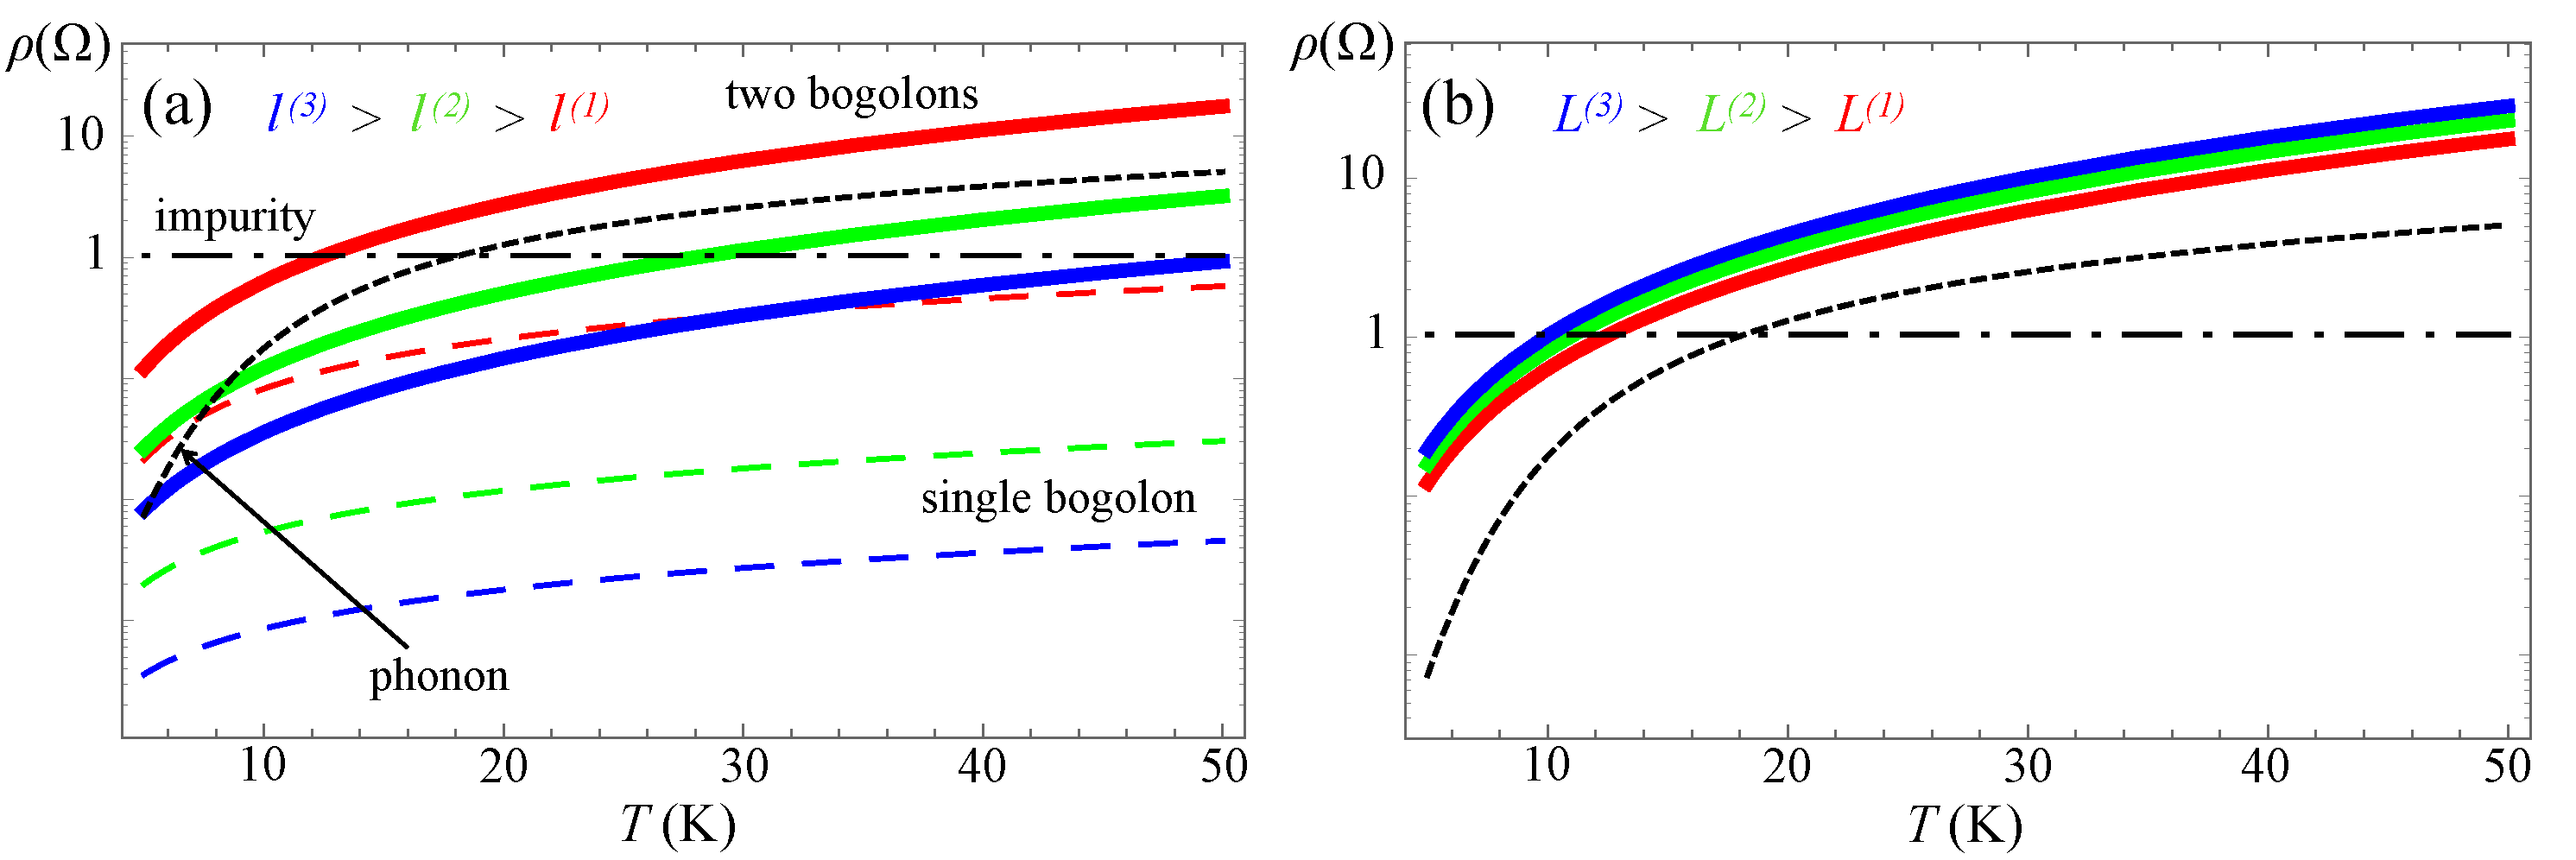
\includegraphics[width=0.99\textwidth]{Fig/AP7/Fig1S.pdf}
\caption[Temperature dependence of single- and double-bogolon resistivity]{Temperature dependence of single- and double-bogolon resistivities at
(a) different interlayer separations: $l=5$ (red), $l=10$ (green), and $l=15$~nm (blue) for fixed $L=10$~$\mu$m,
and at
(b) different sample sizes: $L=10$ (red), $L=100$, and $L=1000$~$\mu$m (blue) for fixed $l=5$~nm.
The density of the MoS$_2$ condensate is taken as $n_c=10^9$~cm$^{-2}$, and the electron density as $n_e=10^{13}$~cm$^{-2}$.
The dashdotted and dashed curves show the corresponding impurity and phonon-mediated resistivities. The figure is taken from~\cite{Villegas:2019aa}.}
\label{AP7_Fig1S}
\end{figure*}
%
%
%

%
% --------------------------------------------
%

\section{Screening}
In this section, we calculate the screening factor $\epsilon_k$. In the presence of a condensate, it takes a usual form~\cite{Fetter:1971aa}
%
\begin{eqnarray}
\epsilon_k=(1-v_k\Pi_k)\left(1-\frac{e_0^2d}{\epsilon_0}P_k\right)-g_k^2\Pi_kP_k,
\end{eqnarray}
%
where $\Pi_k=-m/\pi$ and $P_k=-4Mn_c/k^2$ are the polarization operators for the electrons and exciton condensate, respectively, $v_k=2\pi e_0^2/k$ is the Coulomb interaction between electrons, and $g_k=e_0^2de^{-kl}/(2\epsilon_0)$ is the electron--exciton interaction.
%
After some algebra, we obtain
%
\begin{eqnarray}
\epsilon_k=1+\frac{2}{a_Bk}+\frac{1}{k^2\xi^2}+\frac{2}{a_Bk}\frac{1}{k^2\xi^2}\left(1-\frac{kd}{2}e^{-2kl}\right),
\end{eqnarray}
%
where $a_B$ is the Bohr radius.
%
For $l/d>1$ ,
%
\begin{eqnarray}
1-\frac{kd}{2}e^{-2kl}\approx 1,
\end{eqnarray}
%
and hence we find
%
\begin{eqnarray}
\epsilon_k=\left(1+\frac{2}{a_Bk}\right)\left(1+\frac{1}{k^2\xi^2}\right).
\end{eqnarray}
%
In order to account for the screening in our calculation of resistivity in Appendices A and B, we should simply replace
%
\begin{eqnarray}
|g_k|^2\rightarrow\left|\frac{g_k}{\epsilon_k} \right|^2.
\end{eqnarray}
%

%
% ----------------------------------
%
\section{Validity of the linear spectrum for bogolons}
In this section, we provide a more quantitative analysis of the linear bogolon dispersion approximation.
Bogolon dispersion can be treated as linear if
\begin{eqnarray}
\xi < k^{-1}.
\end{eqnarray}
%
Due to the appearance of the factor
%
\begin{eqnarray}
g_k^2\sim e^{-2lk}
\end{eqnarray}
%
in the integral over $k$, the relevant contribution to the integral is only over the range
%
\begin{eqnarray}
2l<k^{-1}.
\end{eqnarray}
%
The linear spectrum approximation is guaranteed to be valid when:
\begin{eqnarray}
\xi &<& 2l\nonumber\\
\frac{\hbar}{2Ms}&<&2l\nonumber\\
\frac{\hbar}{4Ms}&<&s=\sqrt{\frac{\kappa n_c}{M}}.
\end{eqnarray}
%
This gives us the lower bound of the condensate density as
%
\begin{eqnarray}
n_c>\frac{\hbar^2}{16Ml^2\kappa}\approx 10^8~ \mbox{cm}^{-2},
\end{eqnarray}
%
for which the linear spectrum approximation is valid.
